\documentclass{article}

\usepackage{amsmath}
\usepackage{amssymb}
\usepackage{amsthm}
\usepackage{authblk}
\usepackage[english]{babel}
\usepackage{blkarray}
\usepackage[font=small]{caption}
\usepackage{cite}
\usepackage{graphicx}

% ---- Author affiliations ---- %

\renewcommand\Affilfont{\itshape\small}

% ---- Propositions, lemmas, defintions... ---- %

\newtheorem{algorithm}{Algorithm}
\newtheorem{corollary}{Corollary}
\newtheorem{definition}{Definition}
%\newtheorem{example}{Example}
\newtheorem{lemma}{Lemma}
\newtheorem{proposition}{Proposition}
%\newtheorem{remark}{Remark}


% ---- Special environments (examples and remarks) ---- %

\newcounter{examplecounter}
\newenvironment{example}
{\small\vspace{0.5\baselineskip}
  \refstepcounter{examplecounter}%
  \noindent\textbf{Example \arabic{examplecounter}.}%
}{\vspace{-0.2\baselineskip}\begin{center}%
  $\star$\end{center}\vspace{0.5\baselineskip}}

\newcounter{remarkcounter}
\newenvironment{remark}
{\small\it\vspace{0.5\baselineskip}
  \refstepcounter{remarkcounter}%
  \noindent\textbf{Remark \arabic{remarkcounter}.}%
}{\vspace{0.5\baselineskip}}

\newenvironment{inset}
{\vspace{0.5\baselineskip}\begin{center}}
{\end{center}\vspace{0.5\baselineskip}}


% ---- Macros ---- %

\newcommand{\smA}{\scriptstyle{A}}
\newcommand{\smC}{\scriptstyle{C}}
\newcommand{\smD}{\scriptstyle{D}}
\newcommand{\smE}{\scriptstyle{E}}
\newcommand{\smG}{\scriptstyle{G}}
\newcommand{\smI}{\scriptstyle{I}}
\newcommand{\smS}{\scriptstyle{S}}
\newcommand{\smT}{\scriptstyle{T}}
\newcommand{\smDELz}{\scriptstyle{\Delta_0}}
\newcommand{\smDELs}{\scriptstyle{\Delta_*}}


%---------------------------------------------------------------

\title{Calibrating MEM seeding heuristics}

\author[1,2]{Guillaume J. Filion}
\affil[1]{Genome Architecture, Gene Regulation, Stem Cells and Cancer
Programme, Center for Genomic Regulation (CRG), The Barcelona Institute of
Science and Technology, Dr. Aiguader 88, Barcelona 08003, Spain.}
\affil[2]{University Pompeu Fabra, Doctor Aiguader, 08003 Barcelona,
Spain.}

\date{\today}

%---------------------------------------------------------------
%---------------------------------------------------------------


\begin{document}

\maketitle

\begin{abstract}
The abstract will come later.
\end{abstract}


%---------------------------------------------------------------
%---------------------------------------------------------------

\section{Introduction}
Some introduction

\section{MEM seeds}

We can describe reads as sequences of four possible symbols representing
the state of the local match with the genome. The first symbol,
represented by a black square indicates a sequencing error. This is a
mismatch between the read and the genome so the nucleotide cannot belong
to a correct MEM seed. It either belongs to an incorrect MEM seed, or it
marks the end of a correct MEM seed.

The second symbol, represented by a black square with a white cross
indicates a sequencing error that is also a mismatch for \emph{all} the
duplicates. The nucleotide cannot belong to any MEM seed (correct or not)
so the next MEM seed must start at the following nucleotide. The symbol
`resets' the seeding process, which becomes in the same state as at the
beginning of the read.

The third symbol, represented by an exclamation mark indicates that the
target sequence is the only local match between the read and the genome.
This means that there is at least one mismatch between the read and any
duplicate since the beginning of the current MEM. From that nucleotide,
the MEM will extend forward until the next sequencing error. This means
that two exclamation marks must be separated by either a black square or a
black square with a cross.

The last symbol, represented as a white square indicates all the other
situations. This can mark the beginning but not the end of a MEM.

\begin{figure}[h]
\centering
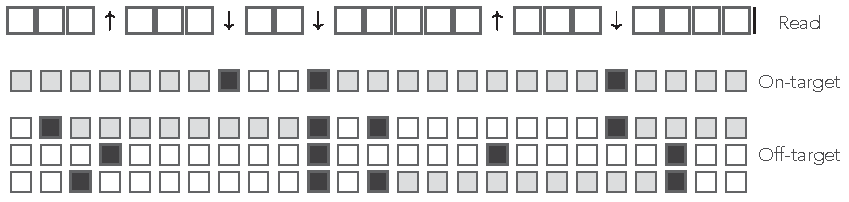
\includegraphics[scale=.9]{sketch_MEM.pdf}
\caption{\textbf{Reads and MEM seeds}. 
Some legend.}
\label{fig:sketch_MEM}
\end{figure}


\begin{equation*}
M(z) =
\begin{blockarray}{ccccccc}
   & \scriptstyle{\blacksquare} & \scriptstyle{\times} 
   & \scriptstyle{(!)_1} & \scriptstyle{(!)_2}
   & \ldots & \scriptstyle{(!)_{\gamma-1}} \\
\begin{block}{c[cccccc]}
\scriptstyle{\blacksquare} & \tilde{A}_\infty(z) & \tilde{B}_\infty(z) &
    r_1(z) & r_2(z) & \ldots & r_{\gamma-1}(z) \\
\scriptstyle{\times} & \tilde{A}_\infty(z) & \tilde{B}_\gamma(z) &
    r_1(z) & r_2(z) & \ldots & r_{\gamma-1}(z) \\
\scriptstyle{(!)_1} & A_{\gamma-1}(z) & B_{\gamma-1}(z) & 0 & 0 &
    \ldots & 0 \\
\scriptstyle{(!)_2} & A_{\gamma-2}(z) & B_{\gamma-2}(z) & 0 & 0 &
    \ldots & 0  \\
\vdots & \vdots & \vdots & \vdots & \vdots & \ddots & \vdots \\
\scriptstyle{(!)_{\gamma-1}} & A_1(z) & B_1(z) & 0 & 0 & \ldots & 0 \\
\end{block}
\end{blockarray}.
\end{equation*}

\begin{eqnarray*}
A_n(z) &=& p (1-(1-\kappa/3)^N) \sum_{m=0}^{n-1} q^mz^{m+1}, \\
\tilde{A}_n(z) &=& p (1-(1-\kappa/3)^N)
    \sum_{m=0}^{n-1} C_m q^mz^{m+1}, \\
B_n(z) &=& p(1-\kappa/3)^N \sum_{m=0}^{n-1} q^mz^{m+1}, \\
\tilde{B}_n(z) &=& p(1-\kappa/3)^N \sum_{m=0}^{n-1} C_m q^mz^{m+1}, \\
r_n(z) &=& (C_{n-1}-C_n) (qz)^n, \\
F_n(z) &=& \sum_{m=0}^n C_m (qz)^m.
\end{eqnarray*}

Define $C_m = \big( 1- (1-(1-\kappa)^m)^N \big)$ as the probability that
during $m$ nucleotides, not all duplicates have collapsed.

\section{Conclusion}
Some conclusion.

\section*{Acknowledgements}

I acknowledge the financial support of the Spanish Ministry of Economy and
Competitiveness (‘Centro de Excelencia Severo Ochoa 2013-2017’, Plan
Nacional BFU2012-37168), of the CERCA Programme~/~Generalitat de
Catalunya, and of the European Research Council (Synergy Grant 609989).


%---------------------------------------------------------------
%---------------------------------------------------------------

\bibliography{references,pubmed}
\bibliographystyle{plain}

%----------------------------------------------------------------

\end{document}

%gs -dNoOutputFonts -sDEVICE=pdfwrite -o out.pdf latex.pdf 
